\documentclass[12pt]{article}

\usepackage{amsmath}
	\numberwithin{equation}{section}
\usepackage{amssymb}
\usepackage{amsthm}
\usepackage{mathtools}
\usepackage{graphicx}
\usepackage{alltt}
\usepackage{ulem}
\usepackage{tikz}
	\usetikzlibrary{arrows,automata}
	\usepackage{tikz-qtree}
\usepackage{xcolor,colortbl}
\usepackage[top=0.7in, left=1in, right=1in, bottom=1in]{geometry}
\usepackage{fancyhdr}
\usepackage{lastpage}

\pagestyle{fancy}
\fancyhf{}
\lhead{Andy Miller, CM1196}
\rhead{\thepage{}/\pageref{LastPage}}

\DeclarePairedDelimiter\floor{\lfloor}{\rfloor}

\title{\textbf{CSSE335 Notes}}
\author{
        Andy Miller \\
        CM 1196 \\
}


%%%%%Useful Commands
\newcommand{\zerovec}{\mathbf{\bar{0}}} %Zero Vector
\newcommand{\vect}[1] {\mathbf{#1}} %Vector Type
\newcommand{\mymatr}[1]{\left(\begin{smallmatrix}#1\end{smallmatrix}\right)} %Inline matrix
\newcommand{\magn}[1]{\lvert\lvert#1\rvert\rvert} %Magnitude
\newcommand{\dotprod}[2]{\vect{#1}^T\vect{#2}} %Dot Product
\newcommand{\innprod}[2]{\langle #1, #2 \rangle} %Inner Product
\newcommand{\proj}[2]{\frac{\innprod{#1}{#2}}{\magn{#2}^2}#2} %Vector Projection
\newcommand{\Nul}{\text{Nul}} %Null space
\newcommand{\Span}{\text{Span}} %Span
\newcommand{\set}[1]{\left\{#1\right\}} %Set brackets
\newcommand{\ceil}[1]{\lceil#1\rceil} %Ceiling function
\newcommand{\abs}[1]{\lvert#1\rvert} %Absolute value
\newcommand{\sep}{\,|\,} %A separator with surrounding spaces
\newcommand{\dd}{\: \mathrm{d}} %Vertical d for integrals
\newcommand{\e}{\mathrm{e}} %Vertical e for math
\newcommand{\scurl}{\mathrm{scurl}} %scurl
\newcommand{\diver}{\mathrm{div}} %div
\newcommand{\del}{\nabla} %Del operator
\newcommand{\lb}{\left\langle} %Left angled bracket for vectors
\newcommand{\rb}{\right\rangle} %Right bracket
\newcommand{\R}{\mathbb{R}} %math R
\newcommand{\Q}{\mathbb{Q}} %math Q
\newcommand{\N}{\mathbb{N}} %math N
\newcommand{\Z}{\mathbb{Z}}


%%%%Partial derivative command
\newcommand{\pderiv}[3][]{
	\ifthenelse{\isempty{#1}}
		{\frac{\partial #2}{\partial #3}}
		{\frac{\partial^{#1} #2}{\partial #3^{#1}}}
} %The #1-th partial derivative of #2 with respect to #3

%%%%Derivative command
\newcommand{\deriv}[3][]{
	\ifthenelse{\isempty{#1}}
		{\frac{d #2}{d #3}}
		{\frac{d^{#1} #2}{d #3^{#1}}}
} %The #1-th derivative of #2 with respect to #3


%%%%%%Changing the look of Greek characters to be "pretty" (Better)
\makeatletter
%\let\old@phi\phi	%Phi -- Commented, I prefer natural \phi for math symbols
%\let\old@varphi\varphi
\let\old@epsilon\epsilon	%Epsilon
\let\old@varepsilon\varepsilon
\let\old@emptyset\emptyset %Empty set
\let\old@varnothing\varnothing
%\let\phi\old@varphi
%\let\varphi\old@phi
\let\epsilon\old@varepsilon
\let\varepsilon\old@epsilon
\let\emptyset\old@varnothing
\let\varnothing\old@emptyset
\makeatother


%%%%%Arrows for rref computation
\newcount\arrowcount
\newcommand\arrows[1]{
        \global\arrowcount#1
        \ifnum\arrowcount>0
                \begin{matrix}
                \expandafter\nextarrow
        \fi
}

\newcommand\nextarrow[1]{
        \global\advance\arrowcount-1
        \ifx\relax#1\relax\else \xrightarrow{#1}\fi
        \ifnum\arrowcount=0
                \end{matrix}
        \else
                \\
                \expandafter\nextarrow
        \fi
}
%%%%%End Arrows

%%%%%Environments
\theoremstyle{theorem}
\newtheorem{theorem}{Theorem}[section]
\theoremstyle{definition}
\newtheorem{definition}{Definition}[section]
\newtheorem{problem}{Problem}[section]
\newtheorem{example}{Example}[section]
\theoremstyle{remark}
\newtheorem*{solution}{Solution}
\newtheorem*{remark}{Remark}

\begin{document}
\maketitle
\tableofcontents
\noindent\rule{\textwidth}{0.4pt}
 
 %%%%% Day 12
\date{March 27, 2015}
\section{Qualitative Measurements Speed}
Assume we have a task of size that needs to be completed.  Let $t_s$ be the time required for the best serial algorithm to complete our task.  Let $t_p$ be the time required for $p$ processors to complete our task.

\begin{definition} We define \textbf{speedup} as
\begin{equation}
s_p = \frac{t_s}{t_p}
\end{equation}
\end{definition}

Ideally, $t_p = \frac{t_s}{p}$ (all work is perfectly divided), but this is almost never the case. Sometimes we cannot divide work evenly (\textbf{load balancing}), and we don't need to account for ``message'' time in serial.  Finally, the best serial algorithms are often dramatically different from the best parallel algorithms (different approaches).  Still, we have this bound on our speedup
\begin{equation}
s_p = \frac{t_s}{t_p} \leq \frac{t_s}{\frac{t_s}{p}} \leq p.
\end{equation}
This means we have at most a $p$ times speedup.

\begin{definition} We measure \textbf{efficiency} as
\begin{equation}
E_p = \frac{s_p}{p} = \frac{\frac{t_s}{t_p}}{p} = \frac{t_s}{p\cdot t_p}.
\end{equation}
\end{definition}

Assume that there is a certain fraction of our work that is inherently serial, $f$.  Then, the amount of time spend on this work is assumed to be $ft_s$.  Then, the time to complete in parallel is
\begin{align}
t_p &= ft_s + \frac{(1-f)t_s}{p}.
\end{align}
This is the best case, where $\frac{(1-f)t_s}{p}$ is a perfectly parallel-ized computataion of the rest of the work.  The speedup of this work is
\begin{equation}
s_p = \frac{t_s}{ft_s + \frac{(1 - f)t_s}{p}} = \frac{pt_s}{pft_s + (1-f)t_s} = \frac{p}{pf + (1 - f)} = \frac{p}{1 + f(p-1)}
\end{equation}
This final result is known as \textbf{Amdahl's Law}:
\begin{equation}
s_p = \frac{p}{1 + f(p - 1)}
\end{equation}
Ideally, we would find the maximum speedup by taking the limit of processors.
\begin{equation}
\lim_{p\to\infty}s_p = \lim_{p\to\infty} \frac{p}{1 + f(p - 1)} = \frac{1}{f}.
\end{equation}
This means that when an algorithm is inherently 5\% serial, it is impossible to make it more than 20 times faster with parallel computation. \\

Amdahl assumes that $t_s$ is fixed, and that we try to decrease $t_p$ with $p$.  Assume instead $t_p$ is fixed, and $t_s$  increases with $p$.  Then, 
\begin{align}
t_s &= ft_s + (1 - f)t_s \\
t_p &= ft_s + \frac{(1 - f)t_s}{t_p} \\
&\vdots \\
s_p &= \frac{t_s}{t_p} \\
&\vdots \\
s_p &= p + (1 - p)ft_s
\end{align}
This was stated by \textbf{Gustafson}: if we add more processes, then do more work.  This causes speedup to be linear in $p$. \\

One thing these models haven't considered is \textbf{communication time}.  We can break parallel processing time into
\begin{equation}
t_p = t_{comp} + t_{comm} = \frac{t_s}{p} + t_{comm}
\end{equation}
Then,
\begin{equation}
s_p = \frac{t_s}{\frac{t_s}{p} + t_{comm}} = \frac{pt_s}{t_s + pt_{comm}}
\end{equation}
If $t_{comm}$ is not insignificant, then we lose a large amount of speedup.  In the real world, communication time will dominate the time consumed by our algorithms.

%%%%% Day 13 or something
\section{Blocking}
\date{March 30, 2015}
Our ``blocking" send isn't that ``blocking" anymore.  Now there's a ``buffer" that is used.  We write what we send to the buffer, and to receive a process goes to the buffer. 

\begin{definition}
A \textbf{locally blocking send} will block \textit{until} we have finished writing into the buffer.  We regain control \textbf{when we can write to the buffer again}.
\end{definition}

\begin{definition}
A \textbf{locally blocking receive} will block until we finish reading data from the buffer.  This functions essentially the same as a regular blocking receive.
\end{definition}

\begin{definition}
A \textbf{synchronous send and receive} fully block the sending process until the receiving process has finished receiving the data.
\end{definition}

\section{Time Estimation}
\begin{equation}
t_p = t_{calc} + t_{comm}
\end{equation}

The calculation time $t_{calc}$ is fairly straightforward, we will count the number of additions/multiplications/etc. 

The time to complete a single communication message is modeled as
\begin{equation}
t_{comm} = t_{startup} + w\cdot t_{data}
\end{equation}
where $t_{startup}$ is a constant startup cost, $w$ is the amount of data, and $t_{data}$ is the data transfer rate.  Unfortunately, the most significant cost is the \textbf{startup cost}

\subsection{Asymptotic Notation}
\begin{definition} $f(x) = O(g(x))$ (\textbf{Big-Oh}) if there exists a constant $c$ such that $0 \leq f(x) \leq cg(x)$ for all ``large" $x$. \end{definition}

\begin{example} $f(x) = 1000x$, $g(x) = x^2$.  $f(0) = g(0)$, $f(1) > g(1)$, $f(2) > g(2)$.  However, $f(1000) = g(1000)$ and for all $x > 1000$, $f(x) < g(x)$.  So, $f(x) = O(g(x))$. 
\begin{center}
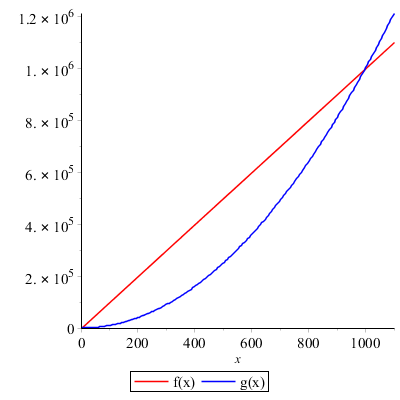
\includegraphics[width=8cm, height=8cm]{./Images/Asymptotic-1.png}
\end{center}
\end{example}

\begin{example} $f(x) = 1000x$, $g(x) = x$.  $f(x) > g(x)$ always, but $f(x) < 1500g(x)$.  So, by the definition, $f(x) = O(g(x))$ (with $c = 1500$).
\begin{center}
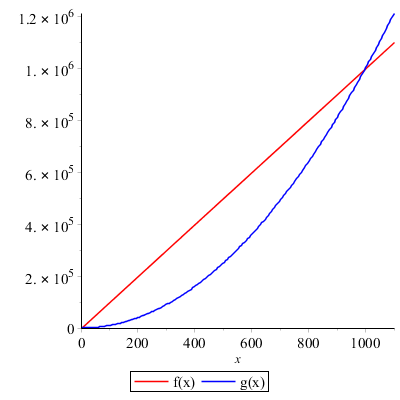
\includegraphics[width=8cm, height=8cm]{./Images/Asymptotic-1.png}
\end{center}
\end{example}

\begin{remark} Big-Oh notation refers to how \textit{fast} a function grows as $x$ becomes large.  \end{remark}

Note that $x = O(x^2)$ but $x^2 \neq O(x)$.  This is because $x^2$ grows faster than all $cx$.  We have an alternate definition for ``grows slower." 

\begin{definition}
$f(x) = \Omega(g(x))$ (\textbf{Big-Omega}) if there exists a constant $c$ such that $f(x) \geq cg(x)$ for all ``large" $x$. 
\end{definition}

Notice that $x = O(x)$, but $x = O(x^2)$ or even $x = O(x^{1000})$.  These last two aren't very descriptive, but still satisfy the definition of $O(g(x))$.  We have a ``tighter" description.

\begin{definition}
$f(x) = \Theta(g(x))$ (\textbf{Big-Theta}) if there exists $c_1, c_2 > 0$ such that $0 \leq c_1g(x) \leq f(x) \leq c_2g(x)$ for all ``large" $x$.  Equivalently, $f(x) = O(g(x))$ and $f(x) = \Omega(g(x))$.
\end{definition}

We want to strive to use Big-Theta as much as possible. 

\subsection{Time Analysis with Processors}
Usually we aren't worried about how time grows with the size of the data so much as how it grows with the numbers of processors.  This immediately brings up one deceptive thing about asymptotic notation: \textit{constants are ignored}.  Parallel computation is mostly dependant on the large constant overhead.  This analysis does not consider that. 

\begin{example} Suppose we have $n$ data, all beginning on processor $p_0$.  We have $P$ processors, and we want $\sum$ data.\end{example}

%%%%% Day 14
\begin{definition} A problem is called \textbf{embarassingly parallel} if it naturally decomposes into independent parts that may be computed in parallel with no (or little) communication between processors. \end{definition}

We have discussed \textbf{MPI\_Gather}, \textbf{MPI\_Scatter} and \textbf{MPI\_AllGather}.

\begin{example} \textbf{Julia Set}.  Let $z$ be a complex number and let $c$ be another complex number.  Define
\begin{align}
z_0 &= z \\
z_{k+1} &= z_k^2 + c
\end{align}
$z$ is in the $c$-Julia set if $\abs{z_k}$ is bounded by all $k$.  
\end{example}

The simplest test to see if $z$ is in the $c$-Julia set is to set an upper bound $M$ and iterations $n$.  If $z_k < M$ for all $k < n$, then we assume $z$ is in the set. 

%%%%% Day 17
We will use an \textbf{escape time criteria} to ``determine'' if something is in the Julia set.  Let $z$, $c$ be given.  Calculate $z_1, \dots, z_{maxiter}$.  If any $\abs{z_i} > M$, then $z \not\in J_c$.  Otherwise, we assume it is.  \\

If we use \textbf{static allocation}, we give each process say 10000 points each.  This could be bad because the first 10,000 (processor 1) could finish much more quickly than the second 10,000 (processor 2).  Instead, we can use \textbf{dynamic allocation}, where processors 

\begin{enumerate}
\item Produce ``julia'' executable. 
\item With infinity options.  Mostly done though! atoi optargs
\item Make complex.h, complex number routines
\subitem Complex struct: add, multiply, norm
\item Forcebyteswap=1 on cluster
\end{enumerate}

%%%%% Day 19
\section{Work Allocation}
\begin{definition} \textbf{Static Work Allocation} is where all tasks are assigned to processors at the very start of program execution. \end{definition}

\begin{definition} \textbf{Dynamic Work Allocation} is where a small amount of work is assigned (statically) to each processor at the start, and there is more work left to do.  When a processor completes its assigned work, more tasks are assigned to it. This is usually referred to as having a \textbf{pool} or processors. \end{definition}

Static allocation gives a well balanced number of tasks for each process.  However, if different tasks are harder to complete (such as with the Julia set), then this does not properly allocate the amount of \textit{work} (and thus time).  Also, static allocation does not take into account the speed of an individual processor (if one is twice as fast, it will finish sooner).

Dynamic allocation is well balanced for time required by each processor (since they all end at roughly the same time).  However, dynamic allocation requires far more communication or overhead.  

\begin{example} Goal: given $N$, produce the array $P$ where $P[i] = 1$ if $i$ is prime, and 0 otherwise. 

Our primality test:  to see if $n$ is prime, try to divide by $2, 3, \dots, n - 1$.  There are far, far better primality tests, but this is very simple to write and will take slightly longer for smaller integers. 

\textbf{Static Allocation:}
\begin{enumerate}
\item Master does no work
\item If there are $w$ processes, worker $i$ will check primality of $k = (i - 1)\frac{N}{w}$ to $k = i\frac{N}{w} - 1$.  
\end{enumerate}
\end{example}

%%%%% Day 21
\section{Partitioning and Divide and Conquer}
There are two main ways to divide up work
\begin{itemize}
\item Data Division (Domain Decomposition, Divide and Conquer)
	\begin{itemize}
	\item Each processor executing the same instructions on a partition of the data
	\item Example: Each process sums $n$ numbers.
	\end{itemize}
\item Instruction Division (Pipelining)
	\begin{itemize}
	\item Each processor executes a few instructions on all of the data
	\item Example: The same idea as a processor pipeline, (Fetch, Decode, Execute, Writeback).  Each processor could be a different stage of the pipeline).
	\end{itemize}
\end{itemize}

\subsection{Bucket Sort}
\begin{definition} (\textbf{Bucket Sort}) Given $n$ numbers to sort, and $m$ buckets with cutoffs $a_1, b_1$, $a_2, b_2$, $\dots$, $a_m, b_m$.  Bucket sort proceeds as follows.  
\begin{enumerate}
\item Partition the data into buckets by putting data $d_i$ into bucket $j$ if $a_j \leq d_i \leq b_j$.  
\item Sort each bucket individually.  
\item There should be (little to) no work required for reassembly.
\end{enumerate}
\end{definition}

\begin{example} Let $d = [-5, 3, 11, 6, -2, 3, 1, 9, -11, 7]$.  We will use 4 buckets: $[-20, -4), [-4, 6), [6, 7), [7, 23)$.  This assignment covers all of the data, and each data point will only be in exactly one bucket.
\begin{enumerate}
\item Partition the data. The buckets are as follows
	\begin{enumerate}
	\item $[-5, -11]$
	\item $[3, -2, -3, 1]$
	\item $[6]$
	\item $[11, 9, 7]$
	\end{enumerate}
\item Sort each bucket individually. Now the buckets rae
	\begin{enumerate}
	\item $[-11, -5]$
	\item $[-3, -2, 1, 3]$
	\item $[6]$
	\item $[7, 9, 11]$
	\end{enumerate}
\item We concatenate the buckets to form a finished list
	\begin{enumerate}
	\item $[-11, -5, -3, -2, 1, 3, 6, 7, 9, 11]$
	\end{enumerate}
\end{enumerate}
\end{example}

\paragraph{Time Complexity} For serial bucket sort. 
\begin{enumerate}
\item Partitioning. $t_{partition} = \Theta(n\cdot\log m)$.  For each $d_i$, we look up the correct bucket.  If the buckets are sorted, then it is a $\log m$ search.
\item Sorting Each Bucket.  A sequential sort in a given bucket depends on the number of elements in the bucket.  If we partition perfectly, each bucket will have exactly $\frac{n}{m}$ elements.  Thus, the time for the sort is $t_{bucket} = \Theta(\frac{n}{m}\log(\frac{n}{m}))$.  However, we must do this for each of the $m$ buckets, so $t_{sort} = \Theta(n\log(\frac{n}{m}))$.  
\item The total time is thus $t_s = t_{partition} + t_{sort} = \Theta(n\log m) + \Theta(n\log \frac{n}{m}) = \Theta(n\log\frac{n}{m})$ since we assume $\frac{n}{m} > n$.
\end{enumerate}
If we have an effective (good distribution) and efficient (quick) way to partition the data, then this is very effective.  However, we cannot pre-process the data to determine good buckets to use (if we spent time on that, we should've just used quicksort instead).  Our goal is to get roughly $\frac{n}{m}$ data per bucket.

For now, we will assume our data is uniformly distributed in $[0, 1]$.  So, for $m$ buckets, we should make the cutoff for bucket $j$ be $\frac{1}{m}(j-1)$ to $\frac{1}{m}j$. 

\paragraph{Parallel Implementation} In parallel, we assign each worker 1 bucket to sort.  We are assuming the data is initially on the master, we have $P$ processors, 1 master, and $m$ workers.  We also want to collect all data on the master again.
\begin{enumerate}
\item Give each worker \textit{all} of the data.  
\item Each processor partitions its portion of data into ``little buckets''
\item Each processor sends its little bucket $i$ to processor $i$ (so processor $i$ has everything in bucket $i$)
\item Each processor sorts its bucket in serial
\item Each processor sends its bucket information back to the master (so the master has the fully sorted list
\end{enumerate}

%%%%% Day 22
\begin{definition} A \textbf{broadcast} the sending of the exact same data from one process to all the others (e.g. the master sends all of the data to each process).  This is implemented as \texttt{MPI\_Bcast}\end{definition}

\begin{definition} A \textbf{gather} is receiving data on one process from all the other processes (e.g. the master receives a result from each other process).  This is implemented as \texttt{MPI\_Gather}. \end{definition}

\paragraph{Time Complexity of Parallel Bucket Sort}
\begin{enumerate}
\item The broadcast: $t_1 = t_{startup} + \abs{d}t_{data}$
\item Partition, takes $t_2 = \frac{\abs{d}}{m}$
\item Correct buckets: $t_3 = m(m)[t_{startup} + t_{data}\frac{d}{m^2}] = m^2t_{startup} + \abs{d}t_{data}$
\item Sort buckets: $t_4 = \frac{\abs{d}}{m}\log(\frac{\abs{d}}{m})$
\item Gather: $t_5 = t_{startup} + \frac{\abs{d}{m}}t_{data}$
\end{enumerate}
We need to add these all together
\begin{align}
t_m &= t_1 + t_2 + t_3 + t_4 + t_5 \\
	&= t_{startup} + \abs{d}t_{data} + \frac{d}{m} + m^2t_{startup} + d + \frac{d}{m}\log(\frac{d}{m}) + mt_{startup} + dt_{data} \\
	&= \Theta(\frac{d\log(\frac{d}{m})}{m})
\end{align}
This is what we wanted, the serial efficiency $\Theta(d\log(\frac{d}{m}))$ but divided by the number of processors.  If we have a good amount of processors relative to the data (we will --- 100 processors vs 1 billion elements), then this scales very well.

\section{Numeric Integration}
\begin{equation}
\int_0^1 \e^{x^2}\, dx
\end{equation}
There is not an antiderivative for $\e^{x^2}$, so we have to find another way to integrate this.  We use Riemann sums.  Specifically, we will use the trapezoidal rule.  
\begin{align}
\int_a^b f(x)\, dx &\approx \delta(\frac{f(x_0) + f(x_1)}{2}) + \frac{\delta}{2}(f(x_1) + f(x_2)) + \frac{\delta}{2}(f(x_2) + f(x_3)) + \dots + \frac{\delta}{2}(f(x_{n-1}) + f(x_n)) \\
	&\approx \delta (\frac{f(a)}{2} + f(x_1) + f(x_2) + \dots + \frac{f(b)}{2})
\end{align}

%%%%% Day 23
\subsection{Adaptive Quadrature}
Let $T(f, a, b, N)$ represent applying the trapezoidal rule from $a$ to $b$ of $f$ with $N$ nodes.
\begin{equation}
T(f, a, b, N) = \delta(\frac{f(a)}{2} + f(x_1) + f(x_2) + \dots + f(x_n) + \frac{f(b)}{2})
\end{equation}
If the problem is worth solving, then $f$ is \textit{ridiculously} difficult to solve.  So, we actually want to minimize the number of function evaluations we have to do.  So, our basic idea is: if
\begin{equation}
\abs{T(f, a, b, N) - T(f, a, b, 2N)} < \epsilon
\end{equation}
then $T(f, a, b, 2N)$ is accepted, otherwise calculate $T(f, a, b, 4N)$ and repeat.  We call this \textbf{adaptive quadrature}. Some pseudocode:
\begin{alltt}
AQ(f, a, b, eps, N):
  approx1 = T(f, a, b, N)
  approx2 = T(f, a, b, 2*N)
  if(abs(approx1 - approx2) < eps) 
    return approx2
  else
    return AQ(f, a, b, eps, 2*N)
\end{alltt}
For some functions, we may be approximating the one half of the function far better than the other half (imagine a function with exponential decay, the beginning has wider variations).  So, instead of simply doubling the nodes, we will integrate the ``left half'' and the ``right half.''  This is truly adaptive because we don't need to get the entire integral in a single iteration (and is easier to parallelize).
\begin{alltt}
AQ(f, a, b, eps, N):
  approx1 = T(f, a, b, N)
  approx2 = T(f, a, b, 2*N)
  if(abs(approx1 - approx2) < eps) 
    return approx2
  else
    L = AQ(f, a, (a+b)/2, eps, N)
    R = AQ(f, (a+b)/2, b, eps, N)
    return L + R
\end{alltt}
This also frees up the processors to do more things.

We ideally want to use dynamic allocation to solve this problem.  However, this is more difficult than the Julia set problem.  With the Julia set, we knew how many tasks their were in total.  In numeric integration, $AQ$ may generate more tasks, so we don't know how many tasks there will be at the start.  Distribution of tasks is more difficult.

\section{N-Body Problem}
Given $N$ stars and initial positions, velocities, and mass, what do they end up after some time?

Let $\vect{x}_i(t)$ be the position of body $B_i$, and $\vect{v}_i(t)$ be the velocity of $B_i$ at time $t$.  Let $m_i$ be the mass of $B_i$, assumed unchanging.  Let $\vect{F}_i$ be the net force acting on $B_i$. Then
\begin{equation}
F_i = m_ia_i = m_iv_i'
\end{equation}
In addition, using the law of gravitation
\begin{equation}
F_1 = g\frac{m_1m_2}{d_{12}^2} + g\frac{m_1m_3}{d_{13}^2} + \dots
\end{equation}
In general, an equation is (writing $d_{ij}^2 = \magn{x_i - x_j}^2$.
\begin{equation}
F_i = gm_i \sum_{j\neq i} \frac{m_j}{\magn{x_i - x_j}^2}
\end{equation}
And so,
\begin{align}
m_i\vect{v}_i' &= Gm_i \sum_{j\neq i} \frac{m_j}{\magn{\vect{x}_i - \vect{x}_j}^2}\cdot\frac{\vect{x}_j - \vect{x}_i}{\magn{\vect{x}_i - \vect{x}_j}} \\
\vect{v}_i' &= G \sum_{j\neq i} \frac{m_j}{\magn{\vect{x}_i - \vect{x}_j}^2}\cdot\frac{\vect{x}_j - \vect{x}_i}{\magn{\vect{x}_i - \vect{x}_j}} \\
\vect{x}_i' &= \vect{v}_i
\end{align}
The last two equations are our system of differential equations. 

\subsection{Euler's Method}
Based on Taylor Series
\begin{equation}
x(t+h) \approx x(t) + h\cdot x'(t)
\end{equation}
This is what we will use to approximate the solution of the $n$-body problem. 

Then we talked about it and I didn't pay attention oops. I was doing other homework, that's right.  It was a long day.

%%%%% Day 25
\section{Pipelining}
\date{April 27, 2015}
Given $d_1, \dots, d_n$ and $x_1, \dots x_n$.  Compute $x_1 + d_1 + d_2 + \dots d_n$, $x_2 + d_1 + d_2 + \dots$, and so on.  Suppose that for some reason we can't just precompute the $\sum d_i$.  I don't know why, but those are the rules.  In serial, we may use the following solution
\begin{alltt}
for i = 1 to n
  compute xi + d1 + d2 + ... + dn
end
\end{alltt}
Specifically, there's this inherently serial ``accumulator,'' but we want to do it several times.  
\begin{alltt}
acc = xi
for j = 1 to m
  acc += dj
end
\end{alltt}
We could break up parts of the function for each process, instead of distributing the function to each process.

Imagine worker $W_j$ has the job ``add $d_j$ to input.''  
\begin{alltt}
global dj

def compute(input):
  return input + dj
  
def worker\_job:
  input = MPI\_receive()
  output = compute(input)
  MPI\_send(output)
\end{alltt}
This puts the job into a \textbf{pipeline}.  After $n$ steps, the pipeline will be full and every processor will be doing something.

To alter this slightly, we are not working with a hardware pipeline; every processor can do the same thing.  Why not have processor 2 begin its input with $x_2$ instead of waiting for $x_1 + d_1$ to start doing anything?  This can fill up the pipeline much more quickly. 

Pipelining is a strategy for breaking up a serial process if we have to do the same process multiple times.  The pseudocode for a workers job is above.  It is fairly simple.  

\subsection{Complexity Analysis}
We mainly analyze ``pipeline cycles,'' which is one transition for a single processor.  In our examples, we need $m + n - 1$ cycles to complete this.  There are $m$ cycles for each processor (for each data), and there is an $n - 1$ ``delay'' before the last cycle starts.  Then, the work of a cycle is $2(t_{startup} + t_{data}) + 1$.  Thus, the total time is
\begin{equation}
t_n = (2(t_{startup} + t_{data}) + 1)(m + n - 1)
\end{equation}
For a large number of jobs $m \gg n$, our cycle efficiency is
\begin{equation}
t_a = \frac{t_n}{m} \approx 2(t_{startup} + t_{data}) + 1
\end{equation}
This means we are getting roughly 1 full job's worth of work done every cycle.

\subsection{Sorting Again}
Suppose we can't partition our data, so we can't use bucket sort.  So, let's do some kind of parallel insertion sort.
\begin{alltt}
for i = 1..n
  for j = 1..length(sorted list)
    is xi the jth largest element?
      if yes, insert xi into sorted list
    else
      loop
\end{alltt}
We can have each processor determine if it has the $j$th largest data.  When it receives data, it checks if $x_j$ is the new $j$th largest element or not.
\begin{alltt}
Recv(data, i-1)
if data < mymax
  send(data, i+1)
else
  send(mymax, i+1)
  mymax = data
\end{alltt}
I'm sure it works somehow.  It totally does.  It doesn't need to know which the first $i - 1$ largest elements are, because workers $1..i-1$ will keep track of that for us.  We just need the max, and that is auto-magically the right work.  Hooray!

%%%%% Day 26
\date{April 28, 2015}
\section{Sieve of Eratosthenes}
I know what this is.  Mark every multiple of $p$ as not prime.  This ``generates'' all the primes up to $n$. 

Do it in parallel.  Pipeline, send some numbers. Use a processor as a filter.

\section{Solving Linear Systems}
\begin{equation}
A\vect{x} = \vect{b}
\end{equation}
This problem is the heart of all modern scientific computing. 

Apparently we talked about this or something?  But I have no notes.  I do know we are doing Gaussian Elimination though, what a boss. 

\subsection{Broadcast Method}
Broadcast row $i$ to processors $i + 1$ to $n$.  Each processor subtracts the correct multiple of $R_i$ from its local row.  
\paragraph{Complexity} 
\begin{itemize}
\item We have $n$ elimination stages.  \\
\item At stage $i$, we broadcast $n - 1$ data to $n - i$ processors
\item There are $n - i$ calculations done to eliminate the rest of the row.
\end{itemize}
The result is 
\begin{align}
\sum_{i=1}^{n-1} \Theta((n - i)\log(n - i)) + \Theta(n - i) \\
	&= \Theta(\sum_{i=1}^{n-i} (n-i)\log(n-i) + (n-i)) \\
	&= \Theta(\sum_{i=1}^{n-i} (n - i)(\log(n - i) + 1)) \\
	&= \Theta(\sum_{i=1}^{n-i} n^2\log(n))
\end{align}
Ta-da

\paragraph{Pipelining}
Pipeline this yo.  Just like, have each processor slowly forward everything along.  It will be wonderful.  If it has useful anyformation, send it ahoy. 

Each processor forwards any useful rows to next processor, and performs any possible eliminations.  The latency of a processor is $\Theta((n-1)n) = \Theta(n)$.  After a little bit of magic, we find that this is \textit{actually} $\Theta(n^2)$ factoring in the necessary work.

Apparently this can also pivot.  That sounds like a mess.

\subsection{Back-Substitution}
Also pretty annoying.  Like, we pretty much just divide, subtract the old answers.  We probably need to broadcast more.  Find $x_n$, then broadcast it.  Use it to find $x_{n-1}$.  Repeat.  In general, the formula for $x_i$ is
\begin{equation}
x_i = \frac{b_i - \sum_{j=i+1}^n a_{ij}x_j}{a_{ii}}
\end{equation}
This is a $\Theta(n^2)$ algorithm in serial.  That means it is the \textit{same} as our parallel Gaussian Elimination.  So, it isn't \textit{that} big of a deal if we don't parallelize it.

But if we want to, we'll run the same pipeline in reverse.
\end{document}